
\chapter{Steam Release}\label{ch:steamrelease}
\renewcommand{\kapitelautor}{Autor: Nils} % todo: replace

%
\subsubsection{Was ist Steam?}\label{subsubsec:Steam-Vorstellung}
\italic{Steam is a platform and app for distributing video games online that also has social media features and community message boards.
It was developed by Valve — the same Valve that created the Half-Life, Counter Strike, and Left4Dead games. It functions like an online shop and a community portal combined and is one of the most popular gaming platforms out there.
You can download the Steam application on Windows, Mac, and Linux; a beta version for ChromeOS is also available. The app lets you purchase games and organize your collection.}\zit{WhatSteam}

Steam ist eine digitale Vertriebsplattform für Computerspiele, die von Valve Corporation entwickelt wurde. Es wurde im Jahr 2003 veröffentlicht und hat sich seitdem zu einer der größten Plattformen für den Verkauf, das Herunterladen und das Spielen von Videospielen entwickelt. Mit Millionen von Nutzern weltweit bietet Steam eine breite Palette von Spielen, von AAA-Titeln bis hin zu kleinen Indiegames, und ermöglicht es Entwicklern, ihre Spiele einem großen Publikum zugänglich zu machen.\cite[vgl.]{Steam}

\subsubsection{Warum ist Steam die beste Wahl für die Veröffentlichung unseres Wild West Indiegames?}\label{subsubsec:Warum-Steam}

Es gibt mehrere Gründe, warum Steam aus unserer Sicht die ideale Plattform für die Veröffentlichung unseres Wild West Indiegames ist:

\begin{liste}
   \item Große Nutzerbasis: Steam hat eine enorme Nutzerbasis von Millionen von Spielern weltweit. Durch die Veröffentlichung auf Steam erhalten wir Zugang zu diesem riesigen Publikum von mehr als einer Milliarde Nutzerkonten, was unsere Reichweite und potenzielle Spielerbasis erheblich erhöht.\cite[vgl.]{Steamzahlen}
   \item Vertriebs- und Marketingunterstützung: Steam bietet verschiedene Tools und Funktionen zur Unterstützung von Vertrieb und Marketing, darunter Werbeaktionen, Rabatte, Empfehlungen und vieles mehr. Diese können uns helfen, die Sichtbarkeit unseres Spiels zu erhöhen und den Umsatz zu steigern.
   \item Entwicklerfreundliche Richtlinien: Steam hat entwicklerfreundliche Richtlinien und bietet faire Konditionen für die Veröffentlichung von Spielen. Im Vergleich zu einigen anderen Plattformen sind die Eintrittsbarrieren niedriger, und die Gebühren sind angemessen.
\end{liste}

\subsubsection{Der Prozess der Veröffentlichung auf Steam}\label{subsubsec:Veröffentlichungsprozess}

Steamworks-Konto erstellen: Der erste Schritt besteht darin, ein Steamworks-Entwicklerkonto zu erstellen. Dazu müssen wir uns auf der Steamworks-Website registrieren und alle erforderlichen Informationen bereitstellen. Dazu gehört die Auswahl des Kontos als Einzelperson, das Ausfüllen eines IRS-Steuerfragebogens, und die Bekanntgabe zahlreicher persönlicher Daten.
\begin{figure}[H]
    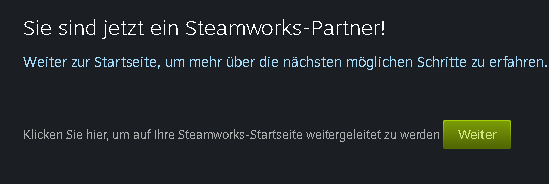
\includegraphics[width=\textwidth]{steamworkspartner.png}
    \caption{Aufnahme ins Partnerprogramm}
\end{figure}

Steam Direct-Gebühr: Bevor man das Spiel auf Steam veröffentlichen konnte, musste man eine einmalige Gebühr von 100 US-Dollar bezahlen. Das Team hat sich dazu entschieden diese Gebühr selbst zu bezahlen. Diese Gebühr deckte die Kosten für die Überprüfung und Verarbeitung des Spiels durch das Steam-Team.
\begin{figure}[H]
    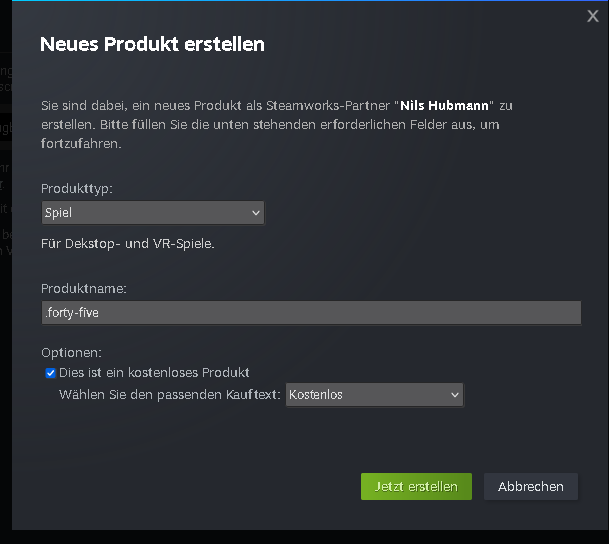
\includegraphics[width=\textwidth]{produkt45.png}
    \caption{Erstellung des Spiels nach Zahlung}
\end{figure}

Verwaltung der Steampage: Während dem gesamten Veröffentlichungsprozess als auch danach, können wir unsere Steampage verwalten und aktualisieren, um sie ansprechend und informativ zu gestalten. Die Bilder werden passend zu unserem Spiel gewählt und sollen spielbeschreibende Inhalte zeigen.
\begin{figure}[H]
    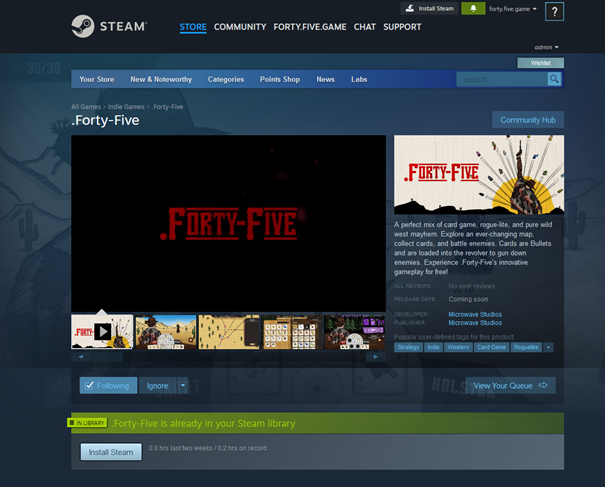
\includegraphics[width=\textwidth]{Steamseite.png}
    \caption{Steamseite}
\end{figure}

Spiel vorbereiten und hochladen: Abschließend muss das Spiel entsprechend den Richtlinien und Vorgaben von Steam vorbereitet sein und alle erforderlichen Dateien, einschließlich Spiel-Assets, Trailer, Screenshots, Videos und Beschreibungen, hochladen. Diese müssen genaueren Anforderung von Steam entsprechen und werden von Mitarbeitern separat in einem Verfahren geprüft.

Überprüfung und Freigabe: Nachdem das Spiel hochgeladen ist, wird es von Steam überprüft, um sicherzustellen, dass es den Richtlinien entspricht und keine technischen Probleme aufweist. Anschließend kann es vom Besitzer freigegeben werden.
\begin{figure}[H]
    
\includegraphics[width=\textwidth]{Steamprozess.png}
    \caption{Steamprozess}
\end{figure}

Insgesamt bietet Steam eine erstklassige Plattform für die Veröffentlichung unseres Wild West Indiegames.
Durch die Nutzung dieser Plattform können wir unser Spiel einem breiten Publikum präsentieren, die Glaubwürdigkeit und das Vertrauen der Spieler stärken und von den
umfangreichen Tools und Funktionen zur Unterstützung von Vertrieb und Marketing profitieren.
Mit einem gut geplanten und durchgeführten Prozess können wir sicherstellen, dass unser Spiel erfolgreich auf Steam veröffentlicht wird und sein volles Potenzial entfaltet.

 \subsubsection{Probleme mit Steam}\label{subsubsec:Steam-Herausforderungen}
Die Veröffentlichung eines Spiels auf Steam kann eine vielversprechende Möglichkeit sein, eine breite Spielerbasis zu erreichen und den Erfolg des Spiels zu steigern. Doch trotz der Potenziale birgt dieser Prozess auch seine Herausforderungen.

Eine der größten Schwierigkeiten sind die langen Wartefristen, die durchlaufen werden müssen, bevor das Spiel auf der Plattform veröffentlicht werden konnte. Diese Wartezeiten dauerten oftmals Wochen, was zu Verzögerungen bei der Markteinführung führt und die Planung erschwert.

Zusätzlich waren die Antwortzeiten des Steam-Supports langsam, was zu Frustration und Verzögerungen bei der Lösung von Problemen geführt hat. Dies war insbesondere problematisch, bei der Veröffentlichung, da es den gesamten Release Plan zerstörte.
Dies passierte da die normalerweise sehr genaue und strenge Steam Dokumentation den Prozess des Early Access Release anders beschrieb als eigentlich vorgesehen, wodurch uns, trotz genauer Befolgung der von Steam bereitgestellten Anweisungen, die Chance auf den Early Access Release genommen wurde.

Ein weiteres generelles Hindernis sind die strengen Dokumentationsanforderungen von Steam. Entwickler müssen eine Vielzahl von Daten und Informationen bereitstellen, was einen umfangreichen und zeitaufwändigen Prozess darstellen kann.

Darüber hinaus ist der Prozess des Hochladens und Konfigurierens des Builds auf Steam oft kompliziert und technisch anspruchsvoll. Dies erfordert nicht nur technisches Know-how, sondern auch Zeit und Ressourcen, um sicherzustellen, dass das Spiel korrekt funktioniert und den Standards von Steam entspricht.

Insgesamt stellen die Schwierigkeiten bei der Veröffentlichung auf Steam eine große Herausforderung dar und erforderten Geduld und Durchhaltevermögen.
Trotz der Hindernisse wird die Veröffentlichung auf Steam jedoch eine lohnende Investition sein, um eine große Spielerbasis zu erreichen und den Erfolg des Spiels zu maximieren.



%

% resets author
\renewcommand{\kapitelautor}{}